\documentclass[10pt,a4paper]{amsart}
\usepackage{amsmath,amssymb,amsthm,graphicx}
\usepackage{amsmath,amssymb,mathtools}
\usepackage{hyperref}
\usepackage{graphicx}
\usepackage{fontspec}
\setmainfont{DejaVu Serif}
\sloppy
\setlength{\emergencystretch}{3em}
\title{Batched maximum-clique computation for all rectangular ranges of unit-disk centres}
\author{J. Mark Keil, Debajyoti Mondal}
\date{doi:10.4230/LIPIcs.SoCG.2025.63; CC BY 4.0}
\begin{document}
\maketitle
\noindent\textit{Editorial scope.} Count only Theorem4. Complete official CC BY4.0 conference author article is retained via publisher mathematical alttext and prose. All three original SVG figures are converted directly to vector PDF without redrawing. The generalized framework includes the bounded-radius disk case as uncounted support; fixed-plane ball extensions are not extra tasks. No mathematical text rewritten.\par\medskip
\noindent\textit{Allowed standard prerequisites (editorial).}\begin{itemize}
\item Bipartite matching, convex geometry and Minkowski sums. Original author exact background, algorithm invocations and bibliography retained; all new source-local geometry is complete.
\end{itemize}\medskip
% BEGIN S1
\par\medskip\noindent\textbf{1 Introduction}\par
% BEGIN S1.p1
A geometric intersection graph consists of a set of geometric objects as vertices and a set of edges that are determined by the intersection of these objects, i.e., two vertices are considered adjacent if and only if the corresponding objects intersect. Geometric objects of different shapes and their intersection graphs are often used to model applied contexts, e.g., unit disks for problems in wireless networks [24, 28], line segments (time intervals) for task scheduling [34], trapezoids for channel routing in VLSI design [23], etc. Many NP-hard graph problems are known to admit polynomial-time solutions on various types of geometric intersection graphs (see e.g., [8, 16]). There also exist cases where a graph problem is known to be NP-hard, but its time complexity status is open for some intersection graph class (see e.g. the open problems posed in [2, 1, 5, 33]). In this paper, we restrict our attention to one such scenario, where the problem of interest is finding a maximum clique, i.e., a maximum subset of pairwise adjacent vertices, and the intersection graph we examine is a disk graph. Here, a disk graph $G$ is an intersection graph of disks in $\mathbb{R}^{2}$, where each vertex of $G$ corresponds to a disk and two vertices are adjacent in $G$ if and only if their disks intersect.
\par
\par
% END S1.p1
% BEGIN S1.p2
The maximum clique problem is NP-hard for many well-known intersection graph classes such as intersection graph of rays [13], grounded strings [33], triangles [3], ellipses [3], and a combination of axis-aligned rectangles and unit disks [7, 21], whereas polynomial-time solvable for circle graphs [36], trapezoid graphs [23], circle trapezoid graphs [23], unit disk graphs [16], axis-aligned rectangle intersection graphs [29], and so on. However, determining the time complexity of computing a maximum clique in a disk graph is a long-standing open question [3, 4, 24]. In a seminal paper published in 1990, Clark, Colbourn, and Johnson [16] gave a polynomial-time algorithm for the case of unit disk graphs. However, the time-complexity question for general disk graphs has remained open since then. Although this was not posed as an open problem in [16], it has long been known to be a challenging problem [4], even before it was explicitly posed as an open problem (e.g., by Fishkin [24], Ambühl and Wagner [3] and Cabello [11, 12]). In fact, the problem has been emphasized in various ways in the literature, e.g., as “an intriguing open question”, as “a notorious open question in computational geometry” [5], as being “elusive with no new positive or negative results” [4], and several times as a “long-standing open problem” [21, 25, 27].
\par
\par
% END S1.p2
% BEGIN S1.p3
Although no polynomial-time exact solution is known for finding a maximum clique in general disk graphs, a 2-approximate solution [3] can be obtained by guessing all stabbing sets of four points. There always exists a stabbing set of at most four points for every set of disks that forms a clique [17, 39, 14]. Therefore, one can take the largest solution obtained from all guesses. However, obtaining a better approximation ratio appears to be a challenge. Cabello [11, 12] even asked whether a 1.99 approximation can be achieved if we restrict the input to disks that have at most two different sizes of radii.
\par
\par
% END S1.p3
% BEGIN S1.p4
Several recent research has shown interesting progress on various fronts of the problem. The $O(n^{4.5})$-time algorithm for finding a maximum clique in a unit disk graph [16], which was improved first to $O(n^{3.5}\log n)$-time [9] and then to $O(n^{3}\log n)$-time [19], has been improved further in SoCG’23 to $O(n^{2.5}\log n)$ [21]. Chan [15] observed that the running time of [21] can be expressed as $O(n\cdot h(m)^{1+o(1)})$, where $h(m)$ is the time to compute a maximum matching in a bipartite graph that has a biclique cover222A biclique cover of a bipartite graph $G$ is a set of complete bipartite subgraphs of $G$ that cover the edges of $G$. The size of the cover is the number of elements in the set. of size $m$, and $m$ in this context is known to be $O(n^{4/3}\mathrm{polylog}(n))$ [31]. One can leverage such a biclique cover to compute a maximum matching in $O(m^{1+o(1)})$ time [22]. Therefore, the overall running time becomes $O(n^{7/3+o(1)})$. In FOCS’18, the authors in [6] gave a QPTAS, a randomized EPTAS (and thus a fixed-parameter-tractable algorithm [7]), and a subexponential algorithm for computing a maximum clique in a disk graph. They also showed how to extend these results for unit ball graphs, which are intersection graphs of 3-dimensional balls of unit radius. In SODA’22, the authors in [35] designed further subexponential-time fixed-parameter-tractable algorithms for many other fundamental graph problems on disk graphs. While the maximum clique problem is open for disk graphs with arbitrary radii, it is NP-hard for ball graphs [6]. The hardness result holds in a very restricted setting with all radii falling within the interval $[1,1+\epsilon]$, $\epsilon>0$, where even a subexponential-time approximation scheme is unlikely unless the exponential-time-hypothesis [30] fails.
\par
\par
% END S1.p4
% BEGIN S1.p5
A rich body of research examined the maximum clique problem in the intersection graph of various types of convex shapes. A $t$-directional convex polygon is a polygon with sides parallel to one of the prespecified $t$ directions. A $t$-directional convex graph is an intersection graph of $t$-directional polygons. The paper in [10] showed that a maximum clique in $k$-directional convex graphs can be solved in time $O(n^{k+3})$ time, and given a geometric representation, this can be improved to $O(n^{k+1})$. The maximum-clique problem can be solved in polynomial time for the intersection graph of unit disks and 2-pancakes [26], where a 2-pancake is defined using a segment on the x-axis. Specifically, a 2-pancake is the Minkowski sum of the unit disk centered at $(0,0)$ and the line segment with endpoints $(x_{1},0)$ and $(x_{2},0)$, i.e., the union of all unit disks with center on the line segment $x_{1}x_{2}$. Bonnet, Grelier, and Miltzow [7] extends the polynomial-time algorithm for unit disks [16] to translates of any fixed convex set. This algorithm does not generalize any further, i.e., no polynomial-time algorithm is known for the translates of two fixed convex sets.
\par
\par
% END S1.p5
% BEGIN S1.SSx1
\par\medskip\noindent\textbf{Our Contribution}\par
We show that a maximum clique in a unit disk graph can be obtained by examining slabs (i.e., regions that are bounded by two parallel lines), whereas all prior algorithms depend on a more constrained lens-shaped region. We show how our new slab-based idea can be extended to compute a maximum clique in polynomial time when the number of different radii sizes is fixed, and even to address the case of ball graphs in some restricted settings. Specifically, we obtain the following results, where in all cases, we assume that an arrangement of disks, i.e., a disk representation of the disk graph, is given as an input.
\par
\par
\par\medskip\noindent\textbf{Disk graph with $k$ Different Sizes of Radii.}\par
We give an $\mathcal{O}^{*}(n^{2k})$-time algorithm, where $\mathcal{O}^{*}$ hides a polynomial factor, to find a maximum clique in a disk graph where $k$ is the number of different types of radii. For every fixed $k$, the running time becomes polynomial. This settles the open question posed by Cabello [11, 12] on whether a polynomial-time algorithm exists when $k=2$.
\par
\par
\par
\par\medskip\noindent\textbf{Range Query in a Unit disk graph.}\par
We show that our slab-based idea can help the range query version of the maximum clique problem, where the input unit disks should be preprocessed such that several queries that may appear at a later time can be answered efficiently. We examine the case of axis-aligned rectangular query, where a maximum clique needs to be reported over disks with centers in the query rectangle. A natural approach for handling rectangular range queries is to precompute the maximum cliques for all possible axis-aligned rectangles (determined by the given disk centers) such that given a query $R$, a solution can be obtained first by identifying the smallest enclosing rectangle $R^{\prime}$ for the disk centers in $R$, and then by a table look-up using $R^{\prime}$. Applying an existing lens-based algorithm on all $O(n^{4})$ possible axis-aligned rectangles determined by the input disk centers takes $O(n^{19/3+o(1)})$ time. In contrast, we can use our slab-based idea to precompute all such solutions in $O(n^{5}\log n)$, achieving a speed up by at least a factor of $n^{4/3}$.
\par
\par
\par
\par\medskip\noindent\textbf{Ball graphs with $k$ Different Sizes of Radii.}\par
Given a set of $n$ balls in the Euclidean plane with $k$ different sizes of radii where the ball centers lie on $r$ parallel planes, we show how to compute a maximum clique in the corresponding ball graph in $\mathcal{O}^{*}(n^{2rk})$ time. For fixed $k$ and $r$, the running time becomes polynomial in $n$. We then show that the restriction of the planes being parallel can be removed as long as the input planes are all perpendicular to a different plane. This result contrasts the known NP-hardness result [5] for finding a maximum clique in a ball graph where the radii of the balls are very close to each other, i.e., in the interval $[1,1+\varepsilon]$, where $\varepsilon>0$.
\par
\par
\par
\par\medskip\noindent\textbf{Intersection graphs of $L$-visible convex polygons.}\par
Given a set $S$ of $n$ convex polygons that are $L$-visible, we show how to find a maximum clique in their intersection graph in $\mathcal{O}^{*}(n^{2k})$-time, where $k$ is the number of distinct shapes in $S$. This strengthens a result in [7]. Here two points $p,q$ in a polygon are called $L$-visible if the axis parallel rectangle with diagonal $pq$ is contained in the polygon. We refer to a polygon $P$ as a $L$-visible polygon if it contains a point from which every point of the polygon is $L$-visible. For example, a disk and a regular hexagon with one side parallel to x-axis are $L$-visible, whereas a triangle is not necessarily an $L$-visible polygon. Our result implies that the maximum clique can be computed in polynomial time in the intersection graph of the translates of a unit disk and a set of fixed axis-aligned rectangles. In contrast, if the number of rectangle shapes is not bounded then the problem is known to be NP-hard, e.g., consider the case of unit disks and axis-aligned rectangles [7, 21].
\par
\par
\par
\par
% END S1.SSx1
% END S1
% BEGIN S2
\par\medskip\noindent\textbf{2 Preliminaries}\par
% BEGIN S2.p1
In this section we discuss some notation and preliminary results.
\par
\par
% END S2.p1
% BEGIN S2.p2
By $D_{a,r}$, we denote a disk with a center at point $a$ and radius $r$. Given a pair of disks $D_{a,r}$ and $D_{b,r^{\prime}}$, we refer to their common intersection region as a lens (Figure 1(a)). Let $G$ be a disk graph. For simplicity, sometimes we say a pair of disks are adjacent in $G$, which means that the disks intersect and their corresponding vertices are adjacent in $G$. By $B_{a,r}$, we denote a ball with a center at point $a$ and radius $r$.
\par
\par
% END S2.p2
% BEGIN S2.F1
\begin{center}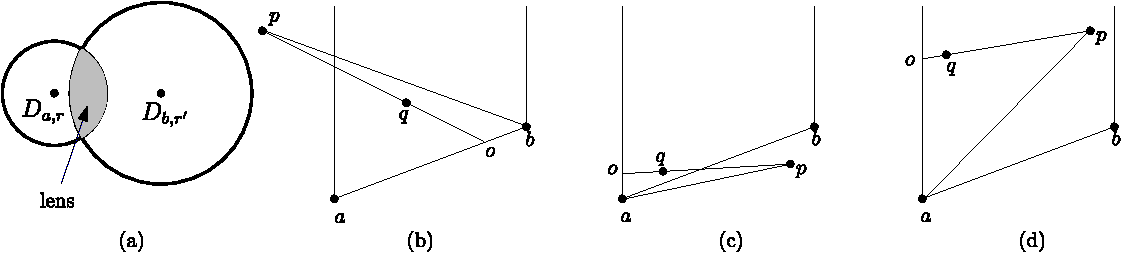
\includegraphics[width=0.7\linewidth,height=0.38\textheight,keepaspectratio]{U1.pdf2svg.pdf}\end{center}
 Figure 1:  Illustration for (a) a lens, (b)–(d) Illustration for Lemma 1.  
% END S2.F1
% BEGIN S2.p3
For a pair of points $a$ and $b$, we denote the line passing through them as $\ell_{ab}$. By $ab$ and $|ab|$ we denote the line segment with endpoints $a,b$ and the Euclidean distance between $a$ and $b$, respectively. By $\ell^{h}_{p}$ and $\ell^{v}_{p}$ we denote the horizontal and vertical lines through a point $p$, respectively. By an upper slab $U_{ab}$ of $ab$, we denote the region above $ab$, which is bounded by the lines $\ell^{v}_{a}$ and $\ell^{v}_{b}$. Similarly, by a lower slab $\overline{U}_{ab}$ we denote the region below $ab$, which is bounded by $\ell^{v}_{a}$ and $\ell^{v}_{b}$.
\par
\par
% END S2.p3
% BEGIN Thmtheorem1
\par\medskip\noindent\textbf{Lemma 1.}\par
Let $ab$ be a line segment and let $U_{ab}$ be the upper slab of $ab$. Let $q$ be a point in $U_{ab}$ and let $p$ be a point (not necessarily in $U_{ab}$) with a $y$-coordinate equal to or larger than the $y$-coordinate of $q$. Then $|pq|\leq\max\{|pa|,|pb|\}$.
\par
\par
\par
% END Thmtheorem1
% BEGIN S2.SS0.SSS0.P0.SPx1
\par\medskip\noindent\textbf{Proof.}\par
We distinguish two scenarios depending on whether $ab$ is vertical or not.
\par
\par
Scenario 1 (The $x$-coordinates of $a$ and $b$ are different): Without loss of generality assume that $a$ has a strictly smaller $x$-coordinate than that of $b$. Since the $y$ coordinate of $p$ is equal to or larger than the $y$-coordinate of $q$, the ray that starts at $p$ and passes through $q$ must hit the boundary of $U_{ab}$. Let $o$ be the point of intersection when the ray exits $U_{ab}$ (e.g., Figure 1(b)–(d)). It suffices to show that $|po|\leq\max\{|pa|,|pb|\}$.
\par
\par
Consider first the case when $o$ lies on $ab$ (e.g., Figure 1(b)). Let $m$ be the point on line $\ell_{ab}$ that minimizes the distance $|pm|$, i.e., $\ell_{pm}$ is perpendicular to $\ell_{ab}$. We now move $o$ away from $m$ along line $\ell_{ab}$ until it hits either $a$ or $b$. Since we are moving $o$ away from $m$, the length $|po|$ increases monotonically, and the largest length it can attain is $\max\{|pa|,|pb|\}$.
\par
\par
Consider now the case when $o$ lies on the vertical sides of $U_{ab}$ (e.g., Figure 1(c)–(d)). We move $o$ downward along the side of $U_{ab}$ until it hits either $a$ or $b$. Since $p$ has a higher $y$-coordinate than $q$, moving $o$ downward increases the length $|po|$ monotonically, and the largest length it can attain is $\max\{|pa|,|pb|\}$.
\par
\par
Scenario 2 (The $x$-coordinates of $a$ and $b$ are the same): In this case, $ab$ is a vertical segment. If $a$ has a smaller $y$-coordinate than that of $b$, then $|pq|\leq|pa|$. Otherwise, $|pq|\leq|pb|$. $\hfill\blacktriangleleft$
\par
\par
\par
% END S2.SS0.SSS0.P0.SPx1
% END S2
% BEGIN S3
\par\medskip\noindent\textbf{3 Maximum Clique in Disk Graphs with $k$ Different Radii}\par
% BEGIN S3.p1
In this section we give an $\mathcal{O}^{*}(n^{2k})$-time algorithm to find a maximum clique in a disk graph where $k$ is the number of different types of radii.
\par
\par
% END S3.p1
% BEGIN S3.p2
We first introduce some notation. Let $\mathcal{D}_{k}$ be a disk graph where the number of different types of radii is at most $k$. For convenience, we denote these different types of radii as $r_{1},r_{2},\ldots,r_{k}$, where for every $1\leq i<j\leq k$, we have $r_{i}<r_{j}$. By a type-$i$ disk we denote a disk of radius $r_{i}$. Let $\mathcal{C}$ be a maximum clique of $\mathcal{D}_{k}$. By $\mathcal{C}_{i}$ we denote a maximal clique in $\mathcal{C}$ where all disks are of type $i$.
\par
\par
% END S3.p2
% BEGIN S3.p3
The idea of the algorithm is as follows. We guess the number of different types of radii that may appear in a maximum clique and we take the maximum over all the solutions computed from these $2^{k}$ guesses. We now describe how a solution is computed for a particular guess for a set of radii that may appear in the maximum clique $\mathcal{C}$. For each disk type $i$, we guess two disk centers $a_{i},b_{i}$ from $\mathcal{C}_{i}$, where $a_{i}$ is the leftmost (i.e., with the smallest $x$-coordinate) and $b_{i}$ is the rightmost (i.e., with the largest $x$-coordinate) over all the disk centers in $\mathcal{C}_{i}$. Note that $a_{i}$ may coincide with $b_{i}$ if $\mathcal{C}_{i}$ contains only one disk, or if the centers of all disks in $\mathcal{C}_{i}$ are on a vertical line. Let $\Psi$ be the set of these $2k$ disks. For every upper slab $U_{a_{i}b_{i}}$, we construct a set $X_{i}$ by taking every disk that has its center in $U_{a_{i}b_{i}}$ and intersects all the disks of $\Psi$. We show that the union of these disks, i.e., $X=(X_{1}\cup X_{2}\cup\ldots\cup X_{k})$, is a clique in $\mathcal{D}_{k}$. Similarly, for each lower slab $\overline{U}_{a_{i}b_{i}}$, we construct a set $Y_{i}$ by taking every disk that has its center in $\overline{U}_{a_{i}b_{i}}$ and intersects all the disks of $\Psi$. We show that their union $Y=(Y_{1}\cup Y_{2}\cup\ldots\cup Y_{k})$ is a clique in $\mathcal{D}_{k}$. Since the disks of $\Psi$ are assumed to be in $\mathcal{C}$, it is straightforward to observe that $\mathcal{C}$ is a subset of the disks in $(\Psi\cup X\cup Y)$. Since the complement of the disk graph determined by the disks $(X\cup Y)$ is a bipartite graph $H$, we can compute the maximum clique $\mathcal{C}$ from a maximum bipartite matching in $H$. It now suffices to show that the disks in $X$ (similarly, the disks in $Y$) are mutually adjacent.
\par
\par
% END S3.p3
% BEGIN Thmtheorem2
\par\medskip\noindent\textbf{Lemma 2.}\par
For every $i,j$, where $1\leq i,j\leq k$, the disks in $X_{i}\cup X_{j}$ are mutually adjacent.
\par
\par
\par
% END Thmtheorem2
% BEGIN S3.SS0.SSS0.P0.SPx1
\par\medskip\noindent\textbf{Proof.}\par
Let $D_{p,r_{i}}$ and $D_{q,r_{j}}$ be two disks, where $p$ belongs to $X_{i}$ and $q$ belongs to $X_{j}$. We now show that $D_{p,r_{i}}$ and $D_{q,r_{j}}$ must mutually intersect.
\par
\par
Consider first the case when $i=j$. Without loss of generality assume that the $y$-coordinate of $p$ is larger than or equal to that of $q$. Then by Lemma 1, $|pq|\leq\max\{|pa_{i}|,|pb_{i}|\}$. By the construction of $X$, the disk $D_{p,r_{i}}$ intersects $D_{a_{i},r_{i}}$ and $D_{b_{i},r_{i}}$. We thus have $|pq|\leq\max\{|pa_{i}|,|pb_{i}|\}\leq 2r_{i}$, and since $p$ and $q$ correspond to type-$i$ disks, they must intersect.
\par
\par
Consider now the case when $i\not=j$.
\par
\par
If the $y$-coordinate of $p$ is larger than or equal to that of $q$, then we apply Lemma 1 to obtain $|pq|\leq\max\{|pa_{j}|,|pb_{j}|\}$. By the construction of $X$, the disk $D_{p,r_{i}}$ intersects $D_{a_{j},r_{j}}$ and $D_{b_{j},r_{j}}$. We thus have $|pq|\leq\max\{|pa_{j}|,|pb_{j}|\}\leq r_{i}+r_{j}$. Consequently, $D_{p,r_{i}}$ and $D_{q,r_{j}}$ mutually intersect.
\par
\par
If the $y$-coordinate of $p$ is smaller than that of $q$, then we apply Lemma 1 by swapping the role of $p$ and $q$, i.e., by using the condition that $p\in U_{a_{i},b_{i}}$ whereas $q$ has a larger $y$-coordinate than that of $p$. We thus have $|pq|\leq\max\{|qa_{i}|,|qb_{i}|\}$. By the construction of $X$, we have $\max\{|qa_{i}|,|qb_{i}|\}\leq r_{i}+r_{j}$. Consequently, $D_{p,r_{i}}$ and $D_{q,r_{j}}$ mutually intersect. $\hfill\blacktriangleleft$
\par
\par
We now consider the running time. There are at most $\binom{n}{0}+\binom{n}{1}+\binom{n}{2}=O(n^{2})$ ways to guess the pair of disks for a particular disk type, irrespective of whether these two disks are distinct or not. Therefore, the number of ways we can guess $k$ pairs is $O(n^{2k})$. For each guess of $k$ pairs, it is straightforward to construct the sets $X$ and $Y$ in $O(kn)$ time. Since the corresponding bipartite graph and its maximum matching can be computed in polynomial time, the overall running time becomes $\mathcal{O}^{*}(n^{2k})$.
\par
\par
The following theorem summarizes the result of this section.
\par
\par
\par\medskip\noindent\textbf{Theorem 3.}\par
Given a set of $n$ disks in the Euclidean plane with $k$ different types of radii, a maximum clique in the corresponding disk graph can be computed in $\mathcal{O}^{*}(n^{2k})$ time.
\par
\par
\par
\par
% END S3.SS0.SSS0.P0.SPx1
% END S3

% BEGIN S4
\par\medskip\noindent\textbf{4 Rectangular Range Query over Unit Disks}\par
% BEGIN S4.p1
In this section, we consider the problem of reporting a maximum clique given a rectangular range query over an arrangement of unit disks. To this end, we show how to compute a maximum clique for every axis-aligned rectangle (determined by the input disk centers) in $O(n^{5}\log n)$ time, which is at least a factor of $n^{4/3}$ faster than applying the algorithm of [21] separately for each axis-aligned rectangle.
\par
\par
% END S4.p1
% BEGIN S4.p2
To better explain such advantages of our technique, we first give an overview of the existing algorithms to compute a maximum clique in a unit disk graph. The idea of Clark, Colbourn, and Johnson’s $O(n^{4.5})$-time algorithm [16] is to guess the farthest pair of vertices $(v,w)$ in the clique, and then to find a maximum clique $C$ that contains both $v$ and $w$. Since $v$ and $w$ are the farthest pair, the set $S$ of vertices that are adjacent to both $v,w$ must lie in a lens-shaped region, i.e., the common intersection region of the two disks centered at $v$ and $w$ with radius $|vw|$. They showed that the lens can be partitioned by the line segment $vw$ into two halves where the disks with centers in the same half are pairwise intersecting. Consequently, the complement of the disk graph corresponding to $S$ is a bipartite graph $H$, and the maximum clique $C$ can be computed by finding a maximum independent set in $H$. The running time for the unit disk case has subsequently been improved to $O(n^{3.5}\log n)$ by using non-trivial data structures [9], then to $O(n^{3}\log n)$ by examining the lenses in a particular order so that the solution for each lens does not need to be computed from scratch [19, 20], and finally, to $O(n\cdot h(m)^{1+o(1)})$ by a combination of divide-and-conquer and plane sweep approach using a circular arc [21, 15]. Here $h(m)$ is the time to compute a maximum matching in $H$, i.e., the complement of the disk graph inside a lens, and $m$ is the size of the biclique cover of $H$. Since $m\in O(n^{4/3}\mathrm{polylog}(n))$ [31] and a maximum matching can be computed using a maximum-flow algorithm in $O(m^{1+o(1)})$ time [22], the running time becomes $O(n^{7/3+o(1)})$. Consider now the scenario of computing a maximum clique for every possible rectangle determined by the input disk centers. Since lenses examined by these algorithms are not necessarily axis-aligned, finding an order of the lenses to compute solutions for the rectangles by dynamic point insertion and deletion appears to be challenging. A straightforward approach that solves each rectangular region independently takes $O(n^{6.33+o(1)})$ time.
\par
\par
% END S4.p2
% BEGIN S4.p3
The idea of our algorithm is to maintain solutions for all possible slabs where one can insert and delete points as necessary to find the solutions for all possible rectangles within the slab. For convenience, we assume that the centers of the disks are in general position, i.e., no two centers have the same $y$-coordinates. We now describe the details.
\par
\par
% END S4.p3
% BEGIN S4.p4
Consider first an alternative (slower) approach that uses slabs to compute a maximum clique that guesses the leftmost and rightmost points $a,b$ of a maximum clique. For every such guess, one can find a maximum clique by considering the set $S$ of disks that are adjacent to both $a,b$ and have their centers in the slab bounded by $\ell^{v}_{a}$ and $\ell^{v}_{b}$. By Lemma 1, the disks of $S$ that have their centers in $U_{ab}$ (similarly, in $\overline{U}_{a,b}$) are mutually adjacent. Consequently, the complement of the disk graph underlying $S$ is a bipartite graph $H$, and a maximum clique can be computed by finding a maximum independent set in $H$.
\par
\par
% END S4.p4
% BEGIN S4.p5
We now consider maintaining the solutions for all possible slabs under point insertion and deletion. Initially, the solution for each slab is set to null. We now sweep the plane upward with two horizontal lines $\ell^{b}$ and $\ell^{u}$ in two phases.
\par
\par
% END S4.p5
% BEGIN S4.p6
In the first phase, $\ell^{b}$ is placed so that it passes through the disk center with the lowest $y$-coordinate, and $\ell^{u}$ is used to sweep the plane upward starting at $\ell_{b}$. Each time $\ell^{u}$ moves to a new point, a point is inserted into the corresponding slabs and their solutions are updated. Every time the horizontal slab between $\ell^{b}$ and $\ell^{u}$ contains the guessed points of a slab (i.e., the two points determining a slab), we obtain a solution for a new rectangular region, and the corresponding solution is stored in a table. It is straightforward to observe that each insertion changes $O(n^{2})$ slabs, and hence we have $O(n^{3})$ insertion operations in total.
\par
\par
% END S4.p6
% BEGIN S4.p7
In the next phase, we sweep the plane upward using $\ell^{b}$. Each time $\ell^{b}$ moves to a new point, a point is deleted from the corresponding rectangular regions we considered in the first phase. A deletion changes $O(n^{3})$ previous solutions, i.e., the solutions corresponding to $O(n^{2})$ slabs and $O(n)$ regions in each slab determined by the positions of $\ell_{b}$. Therefore, we have $O(n^{4})$ deletion operations in total.
\par
\par
% END S4.p7
% BEGIN S4.p8
Each insertion and deletion operation updates existing lenses, each of which is determined by a pair of guessed points. It is known that such updates can be done in $O(n\log n)$ time by performing an alternating path search to update the maximum independent set in the bipartite graph determined by the complement of the disk graph inside the lens [20, 19]. For $O(n^{4})$ update operations, the running time becomes $O(n^{5}\log n)$. By $S[p_{\ell},p_{r},p_{t},p_{b}]$ we denote the size of a maximum clique inside a rectangle $R$ with its left, right, top and bottom sides being determined by the lines through the disk centers $p_{\ell},p_{r},p_{t},p_{b}$, respectively, where $|p_{\ell},p_{r}|$ is at most two units and $p_{\ell},p_{r}$ appear on the left and right sides of $R$. If $|p_{\ell},p_{r}|$ is larger than two units, then $S[p_{\ell},p_{r},p_{t},p_{b}]$ is 0.
\par
\par
% END S4.p8
% BEGIN S4.p9
We now compute a maximum clique for each axis-aligned rectangle determined by the input disk centers. We first compute two sorted orders of the disk centers, one based on increasing $x$-coordinates and the other based on increasing $y$-coordinates. We now use a dynamic programming approach, where the base cases are the entries of $S$, and the $O(n^{4})$ rectangles that do not contain any disk center in their proper interior. The latter can be computed and stored in a table in $O(n^{4})$ time. Let $M[p_{\ell},p_{r},p_{t},p_{b}]$ be the maximum clique of a rectangle $R$ with its left, right, top and bottom sides being determined by the lines through $p_{\ell},p_{r},p_{t},p_{b}$, respectively. Note that the disk centers of the maximum clique may not appear on the sides of $R$. Let $p^{\prime}_{\ell}$ and $p^{\prime}_{r}$ be the disk centers immediately after and before $p_{\ell}$ and $p_{r}$, respectively, which can be determined from the precomputed sorted order. Similarly, $p^{\prime}_{t}$ and $p^{\prime}_{b}$ are the disk centers immediately before and after $p_{t}$ and $p_{b}$, respectively. We now can find a solution using $O(1)$ table look-ups as follows.
\par
\[\begin{aligned}
\displaystyle M[p_{\ell},p_{r},p_{t},p_{b}]{=}\begin{cases}\max\{S[p_{\ell},p_%
{r},p_{t},p_{b}],M[p^{\prime}_{\ell},p_{r},p_{t},p_{b}],\\
\hskip 28.45274ptM[p_{\ell},p^{\prime}_{r},p_{t},p_{b}],M[p_{\ell},p_{r},p^{%
\prime}_{t},p_{b}],\\
\hskip 28.45274ptM[p_{\ell},p_{r},p_{t},p^{\prime}_{b}]\},&\text{if $p_{\ell}$%
 and $p_{r}$ appear on $R$}\\
\max\{M[p^{\prime}_{\ell},p_{r},p_{t},p_{b}],M[p_{\ell},p^{\prime}_{r},p_{t},p%
_{b}],\\
\hskip 28.45274ptM[p_{\ell},p_{r},p^{\prime}_{t},p_{b}],M[p_{\ell},p_{r},p_{t}%
,p^{\prime}_{b}]\},\\
&\text{otherwise.}\\
\end{cases}
\end{aligned}\]
\par
% END S4.p9
% BEGIN S4.p10
Since there are $O(n^{4})$ cells in the table and each entry is computed by $O(1)$ table look-ups which are determined in $O(\log n)$ time, the overall running time remains $O(n^{5}\log n)$.
\par
\par
% END S4.p10

% BEGIN Thmtheorem4
\par\medskip\noindent\textbf{Theorem 4.}\par
Given a set of $n$ unit disks in the Euclidean plane, a maximum clique for every possible axis-aligned rectangle determined by the given disk centers can be computed in $O(n^{5}\log n)$ time.
\par
\par
\par
% END Thmtheorem4

% END S4
% BEGIN S5
\par\medskip\noindent\textbf{5 Maximum Clique in Ball Graphs with $k$ Different Radii}\par
% BEGIN S5.p1
We now give an $\mathcal{O}^{*}(n^{2rk})$-time algorithm for computing a maximum clique in a ball graph, where the centers of the balls are contained in $r$ planes which are all perpendicular to a different plane (Section 5.2). For simplicity, we first consider a scenario when the input planes are parallel to each other (Section 5.1).
\par
\par
% END S5.p1
% BEGIN S5.SS1
\par\medskip\noindent\textbf{5.1 Ball Centers are on $r$ Parallel Planes}\par
Without loss of generality, we assume that the $r$ input planes are parallel to the xy-plane. We first show that a version of Lemma 1 holds in three dimensions, as follows.
\par
\par
\par\medskip\noindent\textbf{Lemma 5.}\par
Let $ab$ be a line segment on a plane $L$, where $L$ is parallel to the xy-plane, and let $U_{ab}$ be the upper slab of $ab$ on $L$. Let $q$ be a point in $U_{ab}$. Let $p$ be a point (not necessarily on $L$) with a $y$-coordinate equal to or larger than the $y$-coordinate of $q$. Then $|pq|\leq\max\{|pa|,|pb|\}$.
\par
\par
\par
\par\medskip\noindent\textbf{Proof.}\par
Let $p^{\prime}$ be the projection of $p$ on $L$ (Figure 2(a)). Then the $y$-coordinate of $p^{\prime}$ is equal to or larger than the $y$-coordinate of $q$. By Lemma 1, $|p^{\prime}q|\leq\max\{|p^{\prime}a|,|p^{\prime}b|\}$ and thus
\par
\[\begin{aligned}
\displaystyle\sqrt{|pq|^{2}-|pp^{\prime}|^{2}}\leq\max\{\sqrt{|pa|^{2}-|pp^{%
\prime}|^{2}},\sqrt{|pb|^{2}-|pp^{\prime}|^{2}}\} \\
\displaystyle\implies & \displaystyle{|pq|^{2}-|pp^{\prime}|^{2}}\leq\max\{{|pa|^{2}-|pp^{\prime}|^{2}%
},{|pb|^{2}-|pp^{\prime}|^{2}}\} \\
\displaystyle\implies & \displaystyle{|pq|}\leq\max\{|pa|,|pb|\}.\ 
\end{aligned}\]
$\hfill\blacktriangleleft$
\par
\par
Let $B_{k}$ be a ball graph with $k$ different types of radii. Similar to Section 3, we guess the number of different types of radii that may appear in a maximum clique and we take the maximum over all the solutions computed from these $2^{k}$ guesses. For each ball type $i$, we guess at most $2r$ ball centers $\{a^{1}_{i},b^{1}_{i}\},\ldots,\{a^{r}_{i},b^{r}_{i}\}$ from $\mathcal{C}_{i}$. Here $a^{j}_{i}$ is the leftmost and $b^{j}_{i}$ is the rightmost over all the ball centers in $\mathcal{C}_{i}$ on the $j$th plane, where $1\leq j\leq r$. Note that $a^{j}_{i}$ may sometimes coincide with $b^{j}_{i}$. Let $\Psi$ be the set of these $2rk$ balls. For every upper slab $U_{a^{j}_{i}b^{j}_{i}}$ on the $j$th plane, we construct a set $X^{j}_{i}$ by taking every ball that has its center in $U_{a^{j}_{i}b^{j}_{i}}$ and intersects all the balls of $\Psi$. We show that the union of these balls, i.e., $X=\bigcup\limits_{1\leq i\leq k}(X^{1}_{i}\cup X^{2}_{i}\cup\ldots\cup X^{r}_{%
i})$, is a clique in $\mathcal{D}_{k}$. Similarly, for each lower slab $\overline{U}_{a_{i}b_{i}}$, we construct a set $Y^{j}_{i}$ by taking every ball that has its center in $\overline{U}_{a^{j}_{i}b^{j}_{i}}$ and intersects all the balls of $\Psi$. We show that their union $Y=\bigcup\limits_{1\leq i\leq k}(Y^{1}_{i}\cup Y^{2}_{i}\cup\ldots\cup Y^{r}_{%
i})$ is a clique in $\mathcal{D}_{k}$. It now suffices to show that the balls in $X$ (similarly, the balls in $Y$) are mutually adjacent.
\par
\par
\begin{center}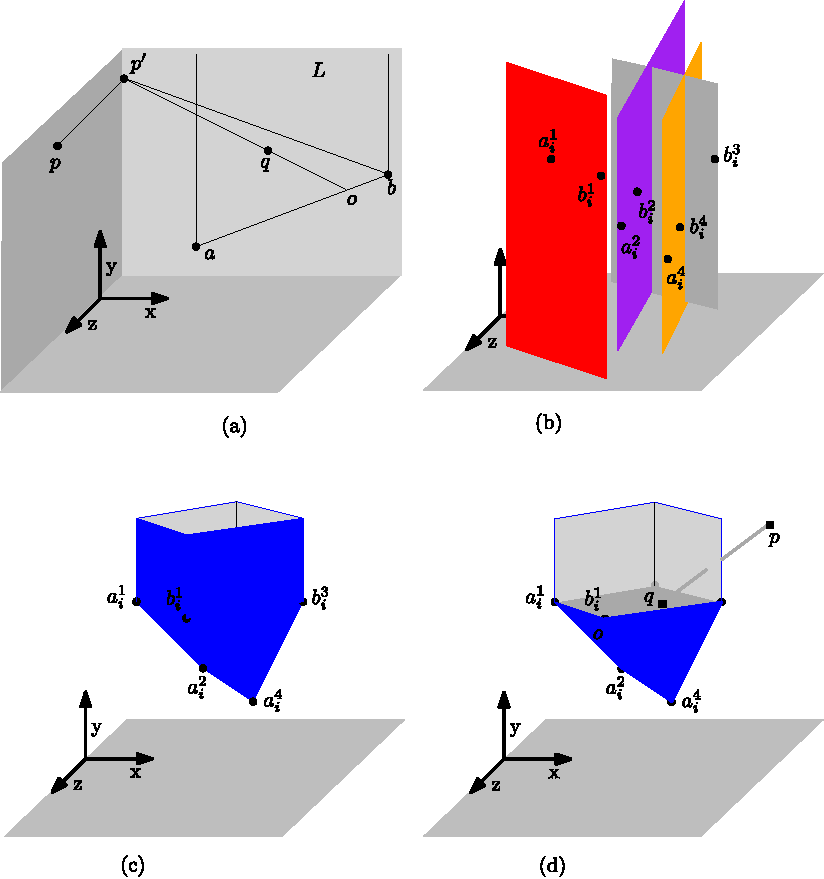
\includegraphics[width=0.7\linewidth,height=0.38\textheight,keepaspectratio]{U2.pdf2svg.pdf}\end{center}
 Figure 2:  Illustration for (a) Lemma 5, and (b)–(d) Lemma 9.   
\par\medskip\noindent\textbf{Lemma 6.}\par
For every $i,j$, where $1\leq i,j\leq k$, the balls in $X^{g}_{i}\cup X^{h}_{j}$, where $1\leq g\leq h\leq r$, are mutually adjacent.
\par
\par
\par
\par
\par\medskip\noindent\textbf{Proof.}\par
Let $B_{p,r_{i}}$ and $B_{q,r_{j}}$ be two balls, where $p$ belongs to $X^{g}_{i}$ and $q$ belongs to $X^{h}_{j}$. We now show that $B_{p,r_{i}}$ and $B_{q,r_{j}}$ must mutually intersect. If $g=h$, then the proof follows from Lemma 2. Therefore, we may assume that $g\not=h$. However, the proof in this case is the same as that of Lemma 2 except that we use Lemma 5 instead of Lemma 1 for the arguments, as follows.
\par
\par
Consider first the case when $i=j$. Without loss of generality assume that the $y$-coordinate of $p$ is larger than or equal to that of $q$. Then by Lemma 5, $|pq|\leq\max\{|pa^{h}_{j}|,|pb^{h}_{j}|\}$. By the construction of $X$, the ball $B_{p,r_{i}}$ intersects $B_{a^{h}_{j},r_{i}}$ and $B_{b^{h}_{j},r_{i}}$. We thus have $|pq|\leq\max\{|pa^{h}_{j}|,|pb^{h}_{j}|\}\leq 2r_{j}$, and since $p$ and $q$ correspond to type-$j$ balls, they must intersect.
\par
\par
Consider now the case when $i\not=j$. If the $y$-coordinate of $p$ is larger than or equal to that of $q$, then we apply Lemma 5 to obtain $|pq|\leq\max\{|pa^{h}_{j}|,|pb^{h}_{j}|\}$. By the construction of $X$, the ball $B_{p,r_{i}}$ intersects $B_{a^{h}_{j},r_{j}}$ and $B_{b^{h}_{j},r_{j}}$. We thus have $|pq|\leq\max\{|pa^{h}_{j}|,|pb^{h}_{j}|\}\leq r_{i}+r_{j}$. Consequently, $B_{p,r_{i}}$ and $B_{q,r_{j}}$ mutually intersect. If the $y$-coordinate of $p$ is smaller than that of $q$, then we apply Lemma 5 by swapping the role of $p$ and $q$, i.e., by using the condition that $p\in U_{a^{g}_{i},b^{g}_{i}}$ whereas $q$ has a larger $y$-coordinate than that of $p$. We thus have $|pq|\leq\max\{|qa^{g}_{i}|,|qb^{g}_{i}|\}$. By the construction of $X$, we have $\max\{|qa^{g}_{i}|,|qb^{g}_{i}|\}\leq r_{i}+r_{j}$. Consequently, $B_{p,r_{i}}$ and $B_{q,r_{j}}$ mutually intersect. $\hfill\blacktriangleleft$
\par
\par
We now consider the running time. For a single plane, there are at most $O(n^{2})$ ways to guess the pair of balls for a particular ball type, and thus $O(n^{2k})$ ways for $k$ pairs considering all types. Since we have $r$ planes, the total number of guesses is $O(n^{2rk})$. For each guess of $rk$ pairs, it is straightforward to construct the sets $X$ and $Y$ in $O(rkn)$ time. Since the the ball graph determined by the balls $(X\cup Y)$ and the corresponding maximum matching can be computed in polynomial time. the running time becomes $\mathcal{O}^{*}(n^{2rk})$.
\par
\par
The following theorem summarizes the result of this section.
\par
\par
\par\medskip\noindent\textbf{Theorem 7.}\par
Given a set of $n$ balls in the Euclidean plane with $k$ different types of radii where the ball centers are contained on $r$ parallel planes, a maximum clique in the corresponding ball graph can be computed in $\mathcal{O}^{*}(n^{2rk})$ time.
\par
\par
\par
\par
\par
% END S5.SS1
% BEGIN S5.SS2
\par\medskip\noindent\textbf{5.2 Ball Centers are on $r$ Planes that are Perpendicular to Another Plane}\par
We now show that the condition for the input planes being parallel to each other can be relaxed as long as the input planes are all perpendicular to a different plane. Without loss of generality assume that the $r$ input planes are perpendicular to the xz-plane (e.g., Figure 2(b)). We first observe the following property of a maximum clique.
\par
\par
\par\medskip\noindent\textbf{Lemma 8.}\par
Let $B_{k}$ be a ball graph with $k$ different radii with centers on $r$ planes that are perpendicular to the xz-plane. Let $\mathcal{C}_{i}$ be all the balls of type $i$ in a maximum clique of $B_{k}$. Let $P$ be the projection of the ball centers in $\mathcal{C}_{i}$ on the xz-plane. Then the convex-hull boundary of $P$ contains at most $2r$ vertices (i.e., they correspond to strictly convex corners).
\par
\par
\par
\par\medskip\noindent\textbf{Proof.}\par
If three points of $P$ come from the same original plane, then they are collinear in the xz-plane, thus only two of them can appear as strictly convex corners on the convex-hull boundary of $P$. Therefore, the $r$ planes can contribute to at most $2r$ vertices in total. $\hfill\blacktriangleleft$
\par
\par
Let $Q$ be a set of points in three dimensions. By a convex hull of $Q$ we denote the smallest convex polyhedra that contains all points in $Q$. A lower (upper) envelope of $Q$ consists of all points that lie at the boundary of the convex hull of $Q$ such that the rays that start at these points and move along the negative y-axis (positive y-axis) do not contain any interior point of the convex hull. An extended lower envelope of $Q$ is a three-dimensional region that consists of the points on the lower envelope and all points that are hit by the rays that start at the lower envelope and move along the positive y-axis. Figure 2(c) illustrates an extended lower envelope. We also define an extended upper envelope of $Q$ symmetrically.
\par
\par
Similar to Section 3, we guess the set of different types of radii that may appear in a maximum clique. For each ball type $i$, we guess at most $2r$ ball centers $\{a^{1}_{i},b^{1}_{i}\},\ldots,\{a^{r}_{i},b^{r}_{i}\}$ from $\mathcal{C}_{i}$, where $a^{j}_{i}$ is the leftmost and $b^{j}_{i}$ is the rightmost over all the ball centers in $\mathcal{C}_{i}$ (e.g., Figure 2(b)) on the $j$th plane. It is straightforward to observe that the convex hull of the projection of the guessed ball centers on the xz-plane contains the projection of all ball centers of $\mathcal{C}_{i}$. Let $\Psi$ be the set of at most $2rk$ balls that we guess over all radii types.
\par
\par
For every extended lower envelope $U_{i}$ for the ball centers guessed for type $i$, we construct a set $\mathcal{X}_{i}$ by taking every ball that has its center in $U_{i}$ and intersects all the balls of $\Psi$. We show that the union of these balls, i.e., $\mathcal{X}=(\mathcal{X}_{1}\cup\mathcal{X}_{2}\cup\ldots\cup\mathcal{X}_{k})$, determines a clique. Similarly, for each extended upper envelope $\overline{U}_{i}$, we construct a set $\mathcal{Y}_{i}$ by taking every ball that has its center in $\overline{U}_{i}$ and intersects all the balls of $\Psi$. We show that their union $\mathcal{Y}=(\mathcal{Y}_{1}\cup\mathcal{Y}_{2}\cup\ldots\cup\mathcal{Y}_{k})$, determines a clique. It now suffices to show that the balls in $\mathcal{X}$ (similarly, the balls in $\mathcal{Y}$) are mutually adjacent.
\par
\par
\par\medskip\noindent\textbf{Lemma 9.}\par
For every $i,j$, where $1\leq i,j\leq k$, the balls in $\mathcal{X}_{i}\cup\mathcal{X}_{j}$ are mutually adjacent.
\par
\par
\par
\par
\par\medskip\noindent\textbf{Proof.}\par
Let $B_{p,r_{i}}$ and $B_{q,r_{j}}$ be two balls, where $p$ belongs to $\mathcal{X}_{i}$ and $q$ belongs to $\mathcal{X}_{j}$. We now show that $B_{p,r_{i}}$ and $B_{q,r_{j}}$ must mutually intersect.
\par
\par
The argument in the rest of the proof works irrespective of whether $i=j$ or not. Without loss of generality assume that the $y$-coordinate of $p$ is larger than or equal to that of $q$. Let $R$ be the ray that starts at $p$ and passes through $q$, and let $o$ be the intersection point of $R$ when $R$ exits the extended lower envelope $U_{i}$. Figure 2(d) illustrates this when $i\not=j$.
\par
\par
Assume first that $o$ hits a face $F$ of the lower envelope, and let $L$ be the plane determined by $F$. Let $m$ be the point of $L$ that minimizes the distance $|pm|$. Since $F$ is convex, moving $o$ away from $m$ on $F$ would increase the length $|po|$ monotonically and hit a vertex $w$ of $F$. Since $B_{p,r_{i}}$ intersects $B_{w,r_{j}}$, and since $|pq|\leq|po|\leq|pw|\leq r_{i}+r_{j}$, the balls $B_{p,r_{i}}$ and $B_{q,r_{j}}$ must intersect.
\par
\par
Assume now that $o$ does not belong to the lower envelope but hits a side $F$ of the extended lower envelope, and let $L$ be the plane determined by $F$. Let $m$ be the point of $L$ that minimizes the distance $|pm|$. Since $F$ is convex, moving $o$ towards negative y-axis and away from $m$ on $F$ would increase the length $|po|$ monotonically and hit a vertex $w$ of $F$. Since $B_{p,r_{i}}$ intersects $B_{w,r_{j}}$, and since $|pq|\leq|po|\leq|pw|\leq r_{i}+r_{j}$, the balls $B_{p,r_{i}}$ and $B_{q,r_{j}}$ must intersect. $\hfill\blacktriangleleft$
\par
\par
The following theorem summarizes the result of this section.
\par
\par
\par\medskip\noindent\textbf{Theorem 10.}\par
Given a set of $n$ balls in the Euclidean plane with $k$ different types of radii where the ball centers are contained on $r$ planes that are perpendicular to a single different plane, a maximum clique in the corresponding ball graph can be computed in $\mathcal{O}^{*}(n^{2rk})$ time.
\par
\par
\par
\par
\par
% END S5.SS2
% END S5
% BEGIN S6
\par\medskip\noindent\textbf{6 Maximum Clique in Disk-Like Graphs}\par
In this section we give an $\mathcal{O}^{*}(n^{2k})$-time algorithm to compute a maximum clique in the intersection graph of $n$ $L$-visible convex polygons with $k$ distinct shapes. Figure 3(a) illustrates an $L$-visible polygon, where every point of the polygon is $L$-visible from a center point $c$.
\par
\par
We first introduce some notation. Let $\mathcal{S}_{k}$ be an intersection graph of $L$-visible polygons, where the number of different types of shapes is at most $k$. For convenience, we denote these shapes as $S_{1},S_{2},\ldots,S_{k}$ and for each shape $S_{i}$, designate a center $c_{i}$, i.e., all points of $S_{i}$ are $L$-visible from $c_{i}$. Let $\mathcal{C}$ be a maximum clique of $\mathcal{S}_{k}$. By $\mathcal{C}_{i}$ we denote a maximal clique in $\mathcal{C}$ where all shapes are of type $i$. We also use the following properties of $L$-visible shapes which are straightforward to verify using the concept of Minkowski sum of two convex polygons [18].
\par
\par
\par\medskip\noindent\textbf{$\blacktriangleright$ Remark 11.}\par
Let $S_{1}$ and $S_{2}$ be two $L$-visible convex shapes with centers $c_{1}$ and $c_{2}$, respectively. Let $\mathcal{R}_{c_{1}}$ be the region that consists of points where $S_{2}$ can be placed to intersect $S_{1}$. Then $\mathcal{R}_{c_{1}}$ is convex (Figure 3(b)).
\par
\par
\par
\begin{center}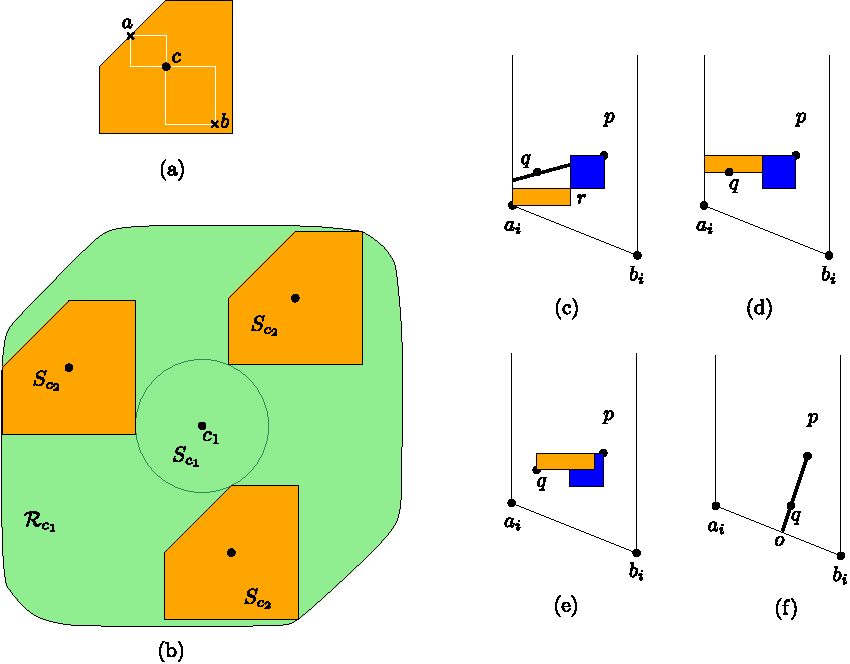
\includegraphics[width=0.7\linewidth,height=0.38\textheight,keepaspectratio]{Lvis.pdf2svg.pdf}\end{center}
 Figure 3: (a) Illustration for $L$-visibility. (b) $\mathcal{R}_{c_{1}}$. (c)–(f) Illustration for the proof of Lemma 12.   
The idea of the algorithm is similar to that of Section 3. We guess the set of different types of shapes that may appear in a maximum clique and we take the maximum over all the solutions computed from these $2^{k}$ guesses. For each type $i$, we guess the leftmost and rightmost shape centers $a_{i}$ and $b_{i}$, respectively, over the shapes in $\mathcal{C}_{i}$. Let $\Psi$ be the set of these $2k$ shapes. For every upper slab $U_{a_{i}b_{i}}$, we construct a set $X_{i}$ by taking every shape that has its center in $U_{a_{i}b_{i}}$ and intersects all the shapes of $\Psi$. We show that the union of these shapes, i.e., $X=(X_{1}\cup X_{2}\cup\ldots\cup X_{k})$, is a clique in $\mathcal{S}_{k}$. Similarly, for each lower slab $\overline{U}_{a_{i}b_{i}}$, we construct a set $Y_{i}$ by taking every shape that has its center in $\overline{U}_{a_{i}b_{i}}$ and intersects all the shapes of $\Psi$. We show that their union $Y=(Y_{1}\cup Y_{2}\cup\ldots\cup Y_{k})$ is a clique in $\mathcal{S}_{k}$. A maximum clique can then be found from a maximum bipartite matching in the complement of the intersection graph of $(X\cup Y)$. The time to compute the graph and the matching is polynomial in $n$ and $m$, where $m$ is the shape complexity, i.e., upper bound on the number of smooth curves on the boundary of a shape.
\par
\par
\par\medskip\noindent\textbf{Lemma 12.}\par
For every $i,j$, where $1\leq i,j\leq k$, the shapes in $X_{i}\cup X_{j}$ are mutually adjacent.
\par
\par
\par
\par\medskip\noindent\textbf{Proof.}\par
Let $S_{q}\in X_{i}$ and $S_{p}\in X_{j}$ be two shapes with centers $q$ and $p$, respectively. We now show that $S_{p}$ and $S_{q}$ must mutually intersect.
\par
\par
Consider first the case when $i=j$, i.e., $p$ and $q$ both belong to the upper slab $U_{a_{i}b_{i}}$. Without loss of generality assume that the $y$-coordinate of $p$ is larger than or equal to that of $q$. We now consider two scenarios.
\par
\par
If the ray starting at $p$ passing through $q$ does not intersect $a_{i}b_{i}$, then assume without loss of generality that it intersects the left side of $U_{a_{i}b_{i}}$ after passing through $q$ (Figure 3(c)). Let $r$ be a point that is common to both $S_{a_{i}}$ and $S_{p}$. Let $R$ be the axis-aligned rectangle with diagonal $rp$. We can then consider moving the center $a_{i}$ along the left side of $U_{a_{i}b_{i}}$ until we reach the $y$-coordinate of $q$, and then move $a_{i}$ horizontally until it coincides with $q$ (Figure 3(d)–(e)). Throughout the process the axis-aligned rectangle with diagonal $a_{i}r$ maintains an intersection region with $R$. Hence $S_{q}$ must intersect $S_{p}$.
\par
\par
If the ray starting at $p$ passing through $q$ intersects $a_{i}b_{i}$ at a point $o$ (Figure 3(f)), then we prove the adjacency of $S_{p}$ and $S_{q}$ as follows. By Remark 11, $\mathcal{R}_{p}$ is convex. Since $S_{p}$ intersects $a_{i}$ and $b_{i}$, $\mathcal{R}_{p}$ also contains $a_{i}$ and $b_{i}$. By the convexity of $\mathcal{R}_{p}$, the segment $a_{i}b_{i}$ belongs to $\mathcal{R}_{p}$. We now move the center $a_{i}$ to $o$ along the line $a_{i}b_{i}$. Since $a_{i}o\in\mathcal{R}_{p}$, throughout the process $S_{a_{i}}$ intersects $S_{p}$. We now move $a_{i}$ from $o$ to $q$ along the line $op$. Since $L$-visible shapes are convex, moving a pair of intersecting $L$-visible shapes closer along the the line determined by their centers keeps them intersected. Therefore, throughout the process $S_{a_{i}}$ maintains an intersection with $S_{p}$. Hence $S_{q}$ must intersect $S_{p}$.
\par
\par
Consider now the case when $i\not=j$. If the $y$-coordinate of $p$ is larger than or equal to that of $q$, then the proof above still applies. The only difference is that $p$ can now be outside of $U_{a_{i}b_{i}}$, but this leaves the above argument the same as we only used the property that the $y$-coordinate of $p$ is larger than or equal to that of $q$. If the $y$-coordinate of $p$ is smaller than that of $q$, then we can swap the role of $p$ and $q$, i.e., by using the condition that $p\in U_{a_{i},b_{i}}$ whereas $q$ has a larger $y$-coordinate than that of $p$. $\hfill\blacktriangleleft$
\par
\par
The running time can now be computed in the same way as in Section 3.
\par
\par
\par\medskip\noindent\textbf{Theorem 13.}\par
Given a set of $n$ $L$-visible convex shapes in the Euclidean plane where the number of distinct shapes is $k$, a maximum clique in the corresponding intersection graph can be computed in $\mathcal{O}^{*}(n^{2k})$ time.
\par
\par
\par
\par
\par
% END S6
% BEGIN S7
\par\medskip\noindent\textbf{7 Direction for Future Research}\par
We gave an $\mathcal{O}^{*}(n^{2k})$-time algorithm to find a maximum clique in a $n$-vertex disk graph with $k$ different radii. Designing faster algorithms is a natural direction to explore. Existing techniques [38] that computes maximum clique on unit disk graphs even when a geometric representation is not given do not generalize to our context. Therefore, finding efficient algorithms when a geometric representation of the disk graph is not given would be interesting.
\par
\par
We showed that given a set of $n$ unit disks, one can compute a maximum clique for each possible axis-aligned rectangle determined by the input disk centers in $O(n^{5}\log n)$ time. Consequently, given a rectangular range query $R$, the maximum clique $C$ inside $R$ can be reported in $O(\log\log n+|C|)$ time, where the $O(\log\log n)$ term is to locate the rectangle $R^{\prime}$ (using range searching data structures [37]) for which a solution is precomputed. Improving the $O(n^{5}\log n)$ running time or establishing tight time-space trade-offs can be interesting.
\par
\par
For ball graphs, we gave an $\mathcal{O}^{*}(n^{2rk})$-time algorithm to find a maximum clique, where $k$ is the number of different radii and the ball centers are contained in $r$ planes that are perpendicular to a single different plane. One may attempt to relax our perpendicularity constraint. The NP-hardness reduction for computing a maximum clique in a ball graph [6] allows for arbitrary radii whereas our result provides polynomial-time algorithms when $r,k\in O(1)$. The case when $k\in o(n)$ can be explored. Finally, can we find a polynomial-time algorithm for computing maximum clique in the intersection graph of convex shapes that are not necessarily $L$-visible, where the number of distinct shapes is fixed?
\par
\par
\par
% END S7
% BEGIN bib
\par\medskip\noindent\textbf{References}\par
\begin{enumerate}
\item[]  [1]  Ranendu Adhikary, Kaustav Bose, Satwik Mukherjee, and Bodhayan Roy.  Complexity of maximum cut on interval graphs.  In Proceedings of the 37th International Symposium on Computational Geometry, (SoCG), volume 189 of LIPIcs, pages 7:1–7:11, 2021.  doi:10.4230/LIPICS.SOCG.2021.7.  
\item[]  [2]  Ranendu Adhikary, Kaustav Bose, Satwik Mukherjee, and Bodhayan Roy.  Complexity of maximum cut on interval graphs.  Discret. Comput. Geom., 70(2):307–322, 2023.  doi:10.1007/S00454-022-00472-Y.  
\item[]  [3]  Christoph Ambühl and Uli Wagner.  The clique problem in intersection graphs of ellipses and triangles.  Theory of Computing Systems, 38(3):279–292, 2005.  doi:10.1007/s00224-005-1141-6.  
\item[]  [4]  J. Bang-Jensen, B. Reed, M. Schacht, R. Šámal, B. Toft, and U. Wagner.  Topics in Discrete Mathematics, Dedicated to Jarik Nešetřil on the Occasion of his 60th birthday, volume 26 of Algorithms and Combinatorics, pages 613–627.  Springer, 2006.  
\item[]  [5]  Marthe Bonamy, Édouard Bonnet, Nicolas Bousquet, Pierre Charbit, Panos Giannopoulos, Eun Jung Kim, Pawel Rzazewski, Florian Sikora, and Stéphan Thomassé.  EPTAS and subexponential algorithm for maximum clique on disk and unit ball graphs.  J. ACM, 68(2):9:1–9:38, 2021.  doi:10.1145/3433160.  
\item[]  [6]  Marthe Bonamy, Edouard Bonnet, Nicolas Bousquet, Pierre Charbit, and Stéphan Thomassé.  EPTAS for max clique on disks and unit balls.  In Mikkel Thorup, editor, Proceedings of the 59th IEEE Annual Symposium on Foundations of Computer Science (FOCS), pages 568–579. IEEE Computer Society, 2018.  doi:10.1109/FOCS.2018.00060.  
\item[]  [7]  Édouard Bonnet, Nicolas Grelier, and Tillmann Miltzow.  Maximum clique in disk-like intersection graphs.  In Proceedings of the 40th IARCS Annual Conference on Foundations of Software Technology and Theoretical Computer Science (FSTTCS 2020), volume 182 of LIPIcs, pages 17:1–17:18. Schloss Dagstuhl – Leibniz-Zentrum für Informatik, 2020.  doi:10.4230/LIPICS.FSTTCS.2020.17.  
\item[]  [8]  Prosenjit Bose, Paz Carmi, J. Mark Keil, Anil Maheshwari, Saeed Mehrabi, Debajyoti Mondal, and Michiel Smid.  Computing maximum independent set on outerstring graphs and their relatives.  Comput. Geom., 103:101852, 2022.  doi:10.1016/j.comgeo.2021.101852.  
\item[]  [9]  Heinz Breu.  Algorithmic aspects of constrained unit disk graphs.  PhD thesis, University of British Columbia, 1996.  
\item[]  [10]  Valentin E Brimkov, Konstanty Junosza-Szaniawski, Sean Kafer, Jan Kratochvíl, Martin Pergel, Paweł Rzążewski, Matthew Szczepankiewicz, and Joshua Terhaar.  Homothetic polygons and beyond: Maximal cliques in intersection graphs.  Discrete Applied Mathematics, 247:263–277, 2018.  doi:10.1016/J.DAM.2018.03.046.  
\item[]  [11]  Sergio Cabello.  Maximum clique for disks of two sizes.  Open problems from Geometric Intersection Graphs: Problems and Directions CG Week Workshop, Eindhoven, June 25, 2015.  
\item[]  [12]  Sergio Cabello.  Open problems presented at the algorithmic graph theory.  Adriatic Coast workshop, Koper, Slovenia, June 16–19, 2015.  
\item[]  [13]  Sergio Cabello, Jean Cardinal, and Stefan Langerman.  The clique problem in ray intersection graphs.  Discret. Comput. Geom., 50(3):771–783, 2013.  doi:10.1007/s00454-013-9538-5.  
\item[]  [14]  Paz Carmi, Matthew J. Katz, and Pat Morin.  Stabbing pairwise intersecting disks by four points.  Discret. Comput. Geom., 70(4):1751–1784, 2023.  doi:10.1007/S00454-023-00567-0.  
\item[]  [15]  Timothy Chan.  Personal communication.  June 6, 2023.  
\item[]  [16]  Brent N. Clark, Charles J. Colbourn, and David S. Johnson.  Unit disk graphs.  Discret. Math., 86(1-3):165–177, 1990.  doi:10.1016/0012-365X(90)90358-O.  
\item[]  [17]  Ludwig Danzer.  Zur lösung des gallaischen problems über kreisscheiben in der euklidischen ebene.  Studia Sci. Math. Hungar, 21(1-2):111–134, 1986.  
\item[]  [18]  Mark De Berg, Marc Van Kreveld, Mark Overmars, and Otfried Schwarzkopf.  Computational geometry: Algorithms and applications.  Springer Science \& Business Media, 2000.  
\item[]  [19]  David Eppstein.  Graph-theoretic solutions to computational geometry problems.  In Christophe Paul and Michel Habib, editors, Proceedings of the 35th International Workshop on Graph-Theoretic Concepts in Computer Science (WG), pages 1–16, 2009.  doi:10.1007/978-3-642-11409-0\_1.  
\item[]  [20]  David Eppstein and Jeff Erickson.  Iterated nearest neighbors and finding minimal polytopes.  Discret. Comput. Geom., 11:321–350, 1994.  doi:10.1007/BF02574012.  
\item[]  [21]  Jared Espenant, J. Mark Keil, and Debajyoti Mondal.  Finding a maximum clique in a disk graph.  In Erin W. Chambers and Joachim Gudmundsson, editors, Proceedings of the 39th International Symposium on Computational Geometry (SoCG), volume 258 of LIPIcs, pages 30:1–30:17. Schloss Dagstuhl – Leibniz-Zentrum für Informatik, 2023.  doi:10.4230/LIPICS.SOCG.2023.30.  
\item[]  [22]  Tomás Feder and Rajeev Motwani.  Clique partitions, graph compression and speeding-up algorithms.  J. Comput. Syst. Sci., 51(2):261–272, 1995.  doi:10.1006/JCSS.1995.1065.  
\item[]  [23]  Stefan Felsner, Rudolf Müller, and Lorenz Wernisch.  Trapezoid graphs and generalizations, geometry and algorithms.  Discret. Appl. Math., 74(1):13–32, 1997.  doi:10.1016/S0166-218X(96)00013-3.  
\item[]  [24]  Aleksei V. Fishkin.  Disk graphs: A short survey.  In Klaus Jansen and Roberto Solis-Oba, editors, Proceedings of Approximation and Online Algorithms, First International Workshop (WAOA), volume 2909 of Lecture Notes in Computer Science, pages 260–264. Springer, 2003.  doi:10.1007/978-3-540-24592-6\_23.  
\item[]  [25]  Nicolas Grelier.  Computing a maximum clique in geometric superclasses of disk graphs.  J. Comb. Optim., 44(4):3106–3135, 2022.  doi:10.1007/S10878-022-00853-2.  
\item[]  [26]  Nicolas Grelier.  Computing a maximum clique in geometric superclasses of disk graphs.  Journal of Combinatorial Optimization, 44(4):3106–3135, 2022.  doi:10.1007/S10878-022-00853-2.  
\item[]  [27]  Nicolas Grelier.  Maximum Clique in Generalisations of Disk Graphs and Plane Geometric Graphs on Degenerate Point Sets.  PhD thesis, ETH Zurich, Zürich, Switzerland, 2022.  doi:10.3929/ETHZ-B-000574739.  
\item[]  [28]  Mark L. Huson and Arunabha Sen.  Broadcast scheduling algorithms for radio networks.  In Proceedings of MILCOM’95, volume 2, pages 647–651. IEEE, 1995.  
\item[]  [29]  Hiroshi Imai and Takao Asano.  Finding the connected components and a maximum clique of an intersection graph of rectangles in the plane.  J. Algorithms, 4(4):310–323, 1983.  doi:10.1016/0196-6774(83)90012-3.  
\item[]  [30]  Russell Impagliazzo, Ramamohan Paturi, and Francis Zane.  Which problems have strongly exponential complexity?  In Proceedings of the 39th Annual Symposium on Foundations of Computer Science (FOCS), pages 653–663. IEEE Computer Society, 1998.  doi:10.1109/SFCS.1998.743516.  
\item[]  [31]  Matthew J. Katz and Micha Sharir.  An expander-based approach to geometric optimization.  SIAM J. Comput., 26(5):1384–1408, 1997.  doi:10.1137/S0097539794268649.  
\item[]  [32]  J. Mark Keil and Debajyoti Mondal.  The maximum clique problem in a disk graph made easy, 2024.  doi:10.48550/arXiv.2404.03751.  
\item[]  [33]  J. Mark Keil, Debajyoti Mondal, Ehsan Moradi, and Yakov Nekrich.  Finding a maximum clique in a grounded 1-bend string graph.  Journal of Graph Algorithms and Applications, 26(4), 2022.  doi:10.7155/JGAA.00608.  
\item[]  [34]  Jon Kleinberg and Éva Tardos.  Algorithm Design.  Addison Wesley, 2006.  
\item[]  [35]  Daniel Lokshtanov, Fahad Panolan, Saket Saurabh, Jie Xue, and Meirav Zehavi.  Subexponential parameterized algorithms on disk graphs (extended abstract).  In Joseph (Seffi) Naor and Niv Buchbinder, editors, Proceedings of the ACM-SIAM Symposium on Discrete Algorithms (SODA), pages 2005–2031. SIAM, 2022.  doi:10.1137/1.9781611977073.80.  
\item[]  [36]  Nicholas Nash and David Gregg.  An output sensitive algorithm for computing a maximum independent set of a circle graph.  Inf. Process. Lett., 110(16):630–634, 2010.  doi:10.1016/j.ipl.2010.05.016.  
\item[]  [37]  Yakov Nekrich.  New data structures for orthogonal range reporting and range minima queries.  In Dániel Marx, editor, Proceedings of the 2021 ACM-SIAM Symposium on Discrete Algorithms (SODA), pages 1191–1205. SIAM, 2021.  doi:10.1137/1.9781611976465.73.  
\item[]  [38]  Vijay Raghavan and Jeremy P. Spinrad.  Robust algorithms for restricted domains.  J. Algorithms, 48(1):160–172, 2003.  doi:10.1016/S0196-6774(03)00048-8.  
\item[]  [39]  L Stachó.  A gallai-féle körletüzési probléma megoldása, mat.  Lapok, 32:19–47, 1981.  
\end{enumerate}
\par
% END bib

\end{document}
